\item
\begin{align}
\begin{split}
\myvec{3 & -1 }\vec{x}&=3
\\
\myvec{9 & -3}\vec{x}&=9
\end{split}
\end{align}
The above equations can be expressed as the matrix equation
\begin{align}
\myvec{3 & -1\\9 & -3} \vec{x} = \myvec{3\\9}
\end{align}
%
Now we converted these matrix equation in augmented matrix form using row reduction
\begin{align}
\myvec{3 & -1 & 3\\9 & -3 & 9} 
\xleftrightarrow {R_2\rightarrow \ \frac{R_2}{3}}\myvec{3 & -1 & 3\\3 & -1 & 3} 
\end{align}
%
Since the rows are linearly dependent, the given set of equations has infinite solutions and the lines are coincident
as can be seen from Fig. \ref{linform/10/fig:SAME LINES.}.
%
\begin{figure}[ht!]
\centering
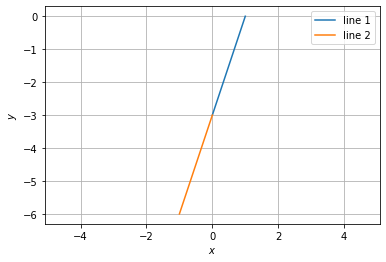
\includegraphics[width=\columnwidth]{solutions/su2021/2/10/FIGURES/SAME-LINE.png}
\caption{SAME-LINES}
\label{linform/10/fig:SAME LINES.}
\end{figure} 
%
\item
\begin{align}
\begin{split}
\myvec{0.2 & 0.3 }\vec{x}&=1.3
\\
\myvec{0.4 & 0.5}\vec{x}&=2.3
\end{split}
\end{align}
The above equations can be expressed as the matrix equation
\begin{align}
\myvec{0.2 & 0.3\\0.4 & 0.5} \vec{x} = \myvec{1.3\\1.4}
\end{align}
%
Now we converted these matrix equation in augmented matrix form using row reduction
\begin{align}
\myvec{0.2 & 0.3 & 1.3\\0.4 & 0.5 & 1.4 } 
\xleftrightarrow {R_2\rightarrow R_2-2R_1}\myvec{0.2 & 0.3 & 1.3\\0 & -0.1 & -0.3} 
\\
%\myvec{0.2 & 0.3 & 1.3} \\0 & 1 & 3
\xleftrightarrow {R_2\rightarrow \frac{R_2}{-0.1}}\myvec{0.2 & 0.3 & 1.3 \\0 & 1 & 3}
\\
%\myvec{0.2 & 0 & 0.4 \\0 & 1 & 3} 
\xleftrightarrow {R_1\rightarrow R_1-0.3R_2}\myvec{0.2 & 0 & 0.4 \\0 & 1 & 3}
\\
%\myvec{1 & 0 & 2\\ 0 & 1 & 3}
\xleftrightarrow {R_1\rightarrow \frac{R_1}{0.2}}\myvec{1 & 0 & 2 \\0 & 1 & 3}
\end{align}
%
Thus, the point of intersection is \myvec{2\\3}, as can be seen from Fig. \ref{linform/10/fig:INTERSECTING LINES.}
%
\begin{figure}[ht!]
\centering
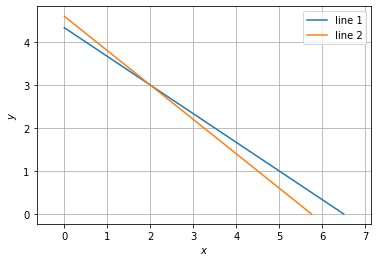
\includegraphics[width=\columnwidth]{solutions/su2021/2/10/FIGURES/INTERSECTING-LINE.png}
\caption{INTERSECTING-LINES}
\label{linform/10/fig:INTERSECTING LINES.}
\end{figure} 


